\section{D. Irga B. Naufal Fakhri}
\subsection{Pemahaman Teori}
\begin{enumerate}
\item Apa itu fungsi library matplotlib

	Matplotlib adalah modul python untuk menggambar plot 2D dengan kualitas tinggi. matplotlib dapat digunakan dalam script python, interpreter python dan ipython, server, dan 6 GUI toolkit. matplotlib berusaha untuk membuat segalanya jadi mudah, dan yang tadinya seperti tidak menjadi mungkin untuk dilakukan. Dengan matplotlib, Anda dapat membuat plots, histograms, spectra, bar charts, errorchards, scatterplots, dan masih banyak lagi.

\item Jelaskan langkah-langkah membuat sumbu X dan Y di matplotlib
\begin{enumerate}
	\item pertama import dulu library matplotlib lalu beri alias plt
	\lstinputlisting[firstline=7, lastline=7]{src/6/1174066/Teori/1174066.py}
	
	\item Kemudian buat variable array x dengan isi terserah anda
	\lstinputlisting[firstline=8, lastline=8]{src/6/1174066/Teori/1174066.py}
	
	\item Lalu buat variable array y juga dengan isi terserah anda yang penting jumlahnya sama dengan variable X
	\lstinputlisting[firstline=9, lastline=9]{src/6/1174066/Teori/1174066.py}
	
	\item Kemudian buat plot berisikan variable x dan y pada modul plt
	\lstinputlisting[firstline=10, lastline=10]{src/6/1174066/Teori/1174066.py}
	
	\item Yang terakhir, munculkan plot yang telah kita buat dengan fungsi show()
	\lstinputlisting[firstline=11, lastline=11]{src/6/1174066/Teori/1174066.py}
\end{enumerate}

\item Jelaskan bagaimana perbedaan fungsi dan cara pakai untuk berbagai jenis(bar,histogram,scatter,line dll) jenis plot di matplotlib

	Perbedaan pada fungsi plot adalah pada bentuk gambar grafik yang dihasilkan pada program dan jenis jenis grafik yang ada pada plot adalah:
\begin{itemize}
	\item Plot
		
	Grafik yang dihasilkan oleh plot ini adalah sebuah garis (line)
	\lstinputlisting[firstline=7, lastline=11]{src/6/1174066/Teori/1174066.py}
	
	\item Bar
	
	Grafik yang dihasilkan oleh bar adalah sebuah bentuk grafik batang (bar) dan cara penggunaan bar adalah menggunakan fungsi bar(variable x, variable y)
	\lstinputlisting[firstline=14, lastline=18]{src/6/1174066/Teori/1174066.py}
	
	\item Histogram
	
	Dalam penggunaaan histogram yaitu menggunakan .hist(variable x, variable y) dengan variable x berisikan data dan variable y berisikan keliapatan yang akan dimunculkan pada histogram
	\lstinputlisting[firstline=21, lastline=24]{src/6/1174066/Teori/1174066.py}
	
	\item Scatter
	
	Grafik yang dihasilkan oleh scatter adalah diagram titik dan cara penggunaannya menggunakan .scatter(variable x, variable y)
	\lstinputlisting[firstline=27, lastline=39]{src/6/1174066/Teori/1174066.py}
	
	\item Stack Plot
	
	Grafik yang dihasilkan oleh stack plot ini hampir sama seperti diagram line, hanya hasil datanya disatuin semua keatasnya dan cara penggunaannya adalah menggunakan .stackplot(variable, variable, variable)
	\lstinputlisting[firstline=41, lastline=58]{src/6/1174066/Teori/1174066.py}
\end{itemize}

\item Jelaskan bagaimana cara menggunakan legend dan label serta kaitannya dengan fungsi tersebut

	Cara menggunakan legend adalah namaObject.legend() dan menambahkan labelnya seperti dibawah ini:
\lstinputlisting[firstline=54, lastline=58]{src/6/1174066/Teori/1174066.py}
Penggunaan legend itu berfungsi untuk memudahkan kita ketika membaca grafik yang kita hasilkan karena kita memberi nama pada data yang ditampilkan sama seperti label kita memberikan nama kepada variable yang dimunculkan di grafik dan membedakan antara variable yang satu dengan yang lain, kita juga bisa menambahkan warna ke label

\item Jelaskan apa fungsi dari subplot di matplotlib, dan bagaimana cara kerja dari fungsi subplot, sertakan ilustrasi dan gambar sendiri dan apa parameternya jika ingin menggambar plot dengan 9 subplot di dalamnya

	Subplot berfungsi untuk menampikan grafik plot pada program yang sama, cara penggunaannya:
\lstinputlisting[firstline=60, lastline=70]{src/6/1174066/Teori/1174066.py}
Cara penggunaannya sebagai contoh saya ambil plt.subplot(221), pada angka 2 yang pertama adalah pembagian keatas kalo kita mau bagi 3 keatas kita isi angka pertama dengan 3, angka 2 yang kedua adalah pembagian kesamping penggunaannya sama kaya angka pertama kalo kita mau ngebagi kesamping 4 kita isi angka kedua 4, dan angka 1 pada angka ketiga itu tempat disimpannya grafik yang akan dimunculkan

\item Sebutkan semua parameter color yang bisa digunakan (contoh: m,c,r,k,... dkk)

	Parameter warna yang bisa digunakan dibagi menjadi 2 tipe:
\begin{itemize}
	\item RGB
	
	Untuk keterangannya sebagai berikut
    R untuk warna Red atau Merah
    G untuk warna Green atau Hijau
    B untuk warna Blue atau Biru
    
    \item CMYK
    
    Untuk keterangannya sebagai berikut
    C untuk warna Cyan atau Biru Muda
    M untuk warna Mangenta atau Merah Tua
    Y untuk warna Yellow Atau Kuning
    K untuk warna Black atau Hitam
\end{itemize}

\item Jelaskan bagaimana cara kerja dari fungsi hist, sertakan ilustrasi dan gambar sendiri

	Untuk histogram kita tidak boleh memiliki is variable x dan y yang sama. Misal x-nya ada 10 nilai sedangkan Y-nya ada 5 nilai, data tersebut tidak menjadi masalah karena pada histogram data yang dimunculkan adalah data rentang dari data variable y. Dan ini adalah contoh dari penggunaan histogram
\lstinputlisting[firstline=82, lastline=87]{src/6/1174066/Teori/1174066.py}

\item Jelaskan lebih mendalam tentang parameter dari fungsi pie diantaranya labels, colors, startangle, shadow, explode, autopct

\begin{itemize}
    \item Label
    
    Label digunakan untuk mempermudah pembaca yaitu memberikan nama pada variable di grafik
    
    \item Color
    
    Warna yang dimunculkan pada setiap data
    
    \item Startangle
    
    Startangle digunakan untuk sudut awal pada diagram pie tersebut
    
    \item Shadow
    
    Shadow(Bayangan) digunakan untuk membuat bayangan pada setiap diagram pie yang menonjol
    
    \item Explode

    Explode digunakan untuk mengeluarkan suatu data agar data tersebut menjadi terlihat lebih menonjol
    
    \item Autopct
    
    Autopct digunakan menyesuaikan berapa angka yang ada dibelakang koma
\end{itemize}
\end{enumerate}

%%%%%%%%%%%%%%%%%%%%%%%%%%%%%%%%%%%%%%%%%%%%%%%%%%%%%%%%%%%%%%%%%%%%%%%%%%%%%%%%%%%%%%%%%%%%%%%%%%%%%%%%%%%%%%%%%%%%%%%%%%

\section{Fanny Shafira Damayanti | 1174069}
\subsection{Pemahaman Teori}
\begin{enumerate}
\item Fungsi Library matplotlib

matplotlib adalah librari plotting 2D Python yang menghasilkan gambar publikasi bermutu di dalam berbagai format hardcopy dan lingkungan interaktif sepanjang platform. matplotlib dapat digunakan di dalam script Python, shell Python dan ipython.

\item Langkah - langkah membuat sumbu X dan Y di matplotlib

caranya yaitu seperti contoh dibawah ini :
\lstinputlisting[firstline=9, lastline=10]{src/6/1174069/Teori/1174069_teori.py}

\item Perbedaan fungsi dan cara pakai untuk berbagai jenis (bar, histogram, scatter,dll) jenis plot di matplotlib

Perbedaannya adalah bentuk bentuk grafik yang akan di tampilkan sesuai dengan perintah yang digunakan pada pemogramannya.

cara pengguna plot tersebut sebagai berikut :

\begin{itemize}
    \item line
    Perintah yang digunakan untuk membuat grafik line sebagai berikut.
    \lstinputlisting[firstline=12, lastline=14]{src/6/1174069/Teori/1174069_teori.py}
	
    \item bar
    Memiliki koordinat X dan Koordinat Y
	\lstinputlisting[firstline=16, lastline=25]{src/6/1174069/Teori/1174069_teori.py}
    
    \item histogram
    Dalam penggunaan plot histogram titik x nya bisa tidak sama dengan titik Y.
    \lstinputlisting[firstline=27, lastline=34]{src/6/1174069/Teori/1174069_teori.py}
   
    \item scatter
   Penggunaan plot scatter atau bisa juga di bilang diagram titik.
   \lstinputlisting[firstline=36, lastline=49]{src/6/1174069/Teori/1174069_teori.py}
    
    \item Stack plot
    Untuk penggunaan stack plot ini seperti diagram line, tapi ada fill colornya,jadi antar line itu bisa berdekatan.
	\lstinputlisting[firstline=82, lastline=92]{src/6/1174069/Teori/1174069_teori.py}
    
\end{itemize}

\item Cara menggunakan legend dan label serta kaitannya dengan fungsi tersebut

Legend digunakan untuk mempermudah dalam membaca grafik, legend itu sendiri berisi info info dari grafik yang ada seperti nama, kemudian bentuk dan warna.
kemudian untuk label itu sendiri digunakan untuk membedakan nama titik X dan titik Y.

Contohnya sebagai berikut :
\lstinputlisting[firstline=20, lastline=22]{src/6/1174069/Teori/1174069_teori.py}

\item Fungsi dari subplot di matplotlib, dan cara kerja dari fungsi subplot sertakan contoh gambarnya

fungsi subplot di matplotlib yaitu untuk bisa membuat lebih dari 1 grafik dalam sebuah program.
Contohnya :
\lstinputlisting[firstline=94, lastline=104]{src/6/1174069/Teori/1174069_teori.py}

\begin{figure}[H]	
    \includegraphics[width=5cm]{figures/6/1174069/Teori/chart.png}
    \centering
    \caption{SubPlot}
\end{figure}

\item Paramater color yang bisa digunakan

\begin{itemize}
    \item Tipe Warna RGB

    R untuk warna Red atau Merah
    G untuk warna Green atau Hijau
    B untuk warna Blue atau Biru
    \item Tipe warna CMYK

    C untuk warna Cyan atau Biru Muda
    M untuk warna Mangenta atau Merah Tua
    Y untuk warna Yellow Atau Kuning
    K untuk warna black atau Hitam
\end{itemize}

\item Cara kerja dari fungsi hist, sertakan ilustrasi dan gambar sendiri

Untuk fungsi histogram ini kedua titik koordinat boleh tidak sama. Misalnya x nya ada 10 nilai sedangkan Y nya ada 5 nilai, itu tidak akan jadi masalah karena diagram ini digunakan untuk mendata usia dari rentang tertentu atau kebutuhan lainnya.
Contoh penggunaan histogram :
\lstinputlisting[firstline=27, lastline=34]{src/6/1174069/Teori/1174069_teori.py}

Contoh grafiknya :
\begin{figure}[H]	
    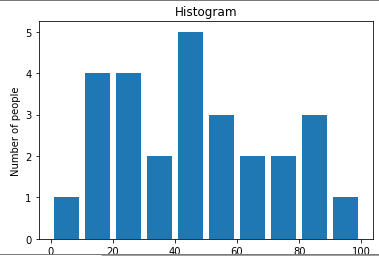
\includegraphics[width=5cm]{figures/6/1174069/Teori/histogram.png}
    \centering
    \caption{Diagram Histogram}
\end{figure}

\item Parameter dari fungsi pie diantaranya labels, colors, startangle, shadow, explode, autopct

\begin{itemize}
    \item label
    Label digunakan untuk mempermudah pembaca dalam membaca diagram pie
    \item color
    warna digunakan untuk membedakan antar data
    \item startangle
    Digunakan untuk sudut yang digunakan untuk memulai diagram pie tersebut
    \item shadow
    bayangan digunakan untuk membuat bayangan dari setiap diagram pie yang menonjol
    \item explode
    explode digunakan untuk mengeluarkan suatu data agar data tersebut terlihat menonjol
    \item autopct
    Digunakan sesuai dengan berapa angka dibelakang koma yang kita inginkan
\end{itemize}

\end{enumerate}

%%%%%%%%%%%%%%%%%%%%%%%%%%%%%%%%%%%%%%%%%%%%%%%%%%%%%%%%%%%%%%%%%%%%%%%%%%%%%%%%%%%%%%%%%%%%%%%%%%%%%%%%%%%%%%%%%%%%%%%%%%%%%%%%%%%%%%%%%%%%%%%%%%%%%%%%%%%%%%%%%%%%%%%%%%%%%%%%%%%%%%%%%%%%%%%%%%%
\section{Tia Nur Candida | 1174086}
\subsection{Teori}
\subsubsection{Soal No. 1}
\hfill \break
Apa itu fungsi library matplotlib?

\hfill \break
Matplotlib merupakan library plotting 2D Python yang menghasilkan gambar publikasi bermutu di dalam berbagai format hardcopy dan lingkungan interaktif di berbagai platform.
Fungsi dari Matplotlib yaitu sebagai pembuat grafik di berbagai platform, seperti Python dan Jupyter. Grafik yang dibuat menggunakan Matplotlib dapat dibuat dalam berbagai bentuk, seperti grafik garis, batang, lingkaran, histogram, dan sebagainya.

\subsubsection{Soal No. 2}
\hfill \break
Jelaskan langkah-langkah membuat sumbu X dan Y di matplotlib!

\begin{enumerate}
	\item Pertama import library Matplotlib.	
	\lstinputlisting[firstline=2, lastline=2]{src/6/1174086/1174086.py}
	
	\item Buat variabel x yang menampung list untuk sumbu x dan variabel y yang menampung list untuk sumbu y.	
	\lstinputlisting[firstline=4, lastline=5]{src/6/1174086/1174086.py}
	
	\item Panggil fungsi plot dan isi parameter pertama dengan variabel x dan parameter kedua dengan variabel y.
	\lstinputlisting[firstline=7, lastline=7]{src/6/1174086/1174086.py}	

	\item Lalu panggil plot tadi dengan memanggil fungsi show.
	\lstinputlisting[firstline=9, lastline=9]{src/6/1174086/1174086.py}
	
\end{enumerate}

 
\subsubsection{Soal No. 3}
\hfill \break
Jelaskan bagaimana perbedaan fungsi dan cara pakai untuk berbagai jenis(bar, histogram ,scatter ,line, dll) jenis plot di matplotlib!

\begin{enumerate}
	\item \textbf{Bar Graph}
	
	Perbedaan bar graph dengan jenis plot yang lain adalah bar graph menggunakan bar atau batang-batang untuk membandingkan data di antara berbagai kategori.
	
	
	\item \textbf{Histogram}
	
	Perbedaan histogram dengan jenis plot yang lain adalah histogram akan membuat plot dimana plot yang dimunculkan merupakan gabungan dari beberapa data yang telah dikelompokkan.
	
	
	
	\item \textbf{Scatter Plot}
	
	Perbedaan scatter plot dengan jenis plot lain adalah scatter plot menampilkan data sebagai kumpulan titik, masing-masing memiliki nilai satu variabel yang menentukan posisi pada sumbu horizontal dan nilai variabel lain menentukan posisi pada sumbu vertikal.
	
	
	
	\item \textbf{Area Plot}
	
	Perbedaan area plot dengan jenis plot lain adalah area plot digunakan untuk melacak perubahan dari waktu ke waktu untuk dua atau lebih kelompok terkait yang membentuk satu kategori secara keseluruhan.
	
		
	\item \textbf{Pie Plot}
	
	Perbedaan pie plot dengan jenis plot lain adalah pie plot digunakan untuk menunjukkan persentase atau data proporsional di mana setiap potongan pie mewakili kategori.
	
		
	\item \textbf{Line Graph}
	
	Perbedaan line graph dengan jenis plot lain adalah line graph menampilkan diagram dalam bentuk garis.
	
	
	
	
	
\end{enumerate}

\subsubsection{Soal No. 4}
\hfill \break
Jelaskan bagaimana cara menggunakan legend dan label serta kaitannya dengan fungsi tersebut!

\begin{enumerate}
	\item Untuk menggunakan legend definisikan parameter label di tiap fungsi plot. Parameter label digunakan untuk memberikan label pada line sebagai pembeda antar line.
	
	\lstinputlisting[caption = Kode program menggunakan parameter label dengan Matplotlib., firstline=19, lastline=20]{src/6/1174086/1174086.py}
	
	\item Kemudian panggil fungsi legend.
	
	\lstinputlisting[caption = Kode program memanggil fungsi legend dengan Matplotlib., firstline=24, lastline=24]{src/6/1174086/1174086.py}
\end{enumerate}

\hfill \break
\textbf{Kode Program}

\lstinputlisting[caption = Kode program membuat diagram menggunakan Matplotlib., firstline=13, lastline=26]{src/6/1174086/1174086.py}

\hfill \break
\textbf{Hasil Compile}

\begin{figure}[H]
	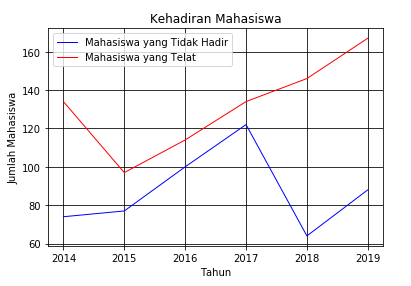
\includegraphics[width=12cm]{figures/6/1174086/4.png}
	\centering
	\caption{Hasil compile membuat diagram menggunakan Matplotlib.}
\end{figure}

\subsubsection{Soal No. 5}
\hfill \break
Jelaskan apa fungsi dari subplot di matplotlib, dan bagaimana cara kerja dari fungsi subplot, sertakan ilustrasi dan gambar sendiri dan apa parameternya jika ingin menggambar plot dengan 9 subplot di dalamnya!

\hfill \break
Fungsi subplot adalah untuk membuat beberapa plot di dalam satu gambar.
\hfill \break
Cara kerja subplot, yaitu fungsi subplot memiliki parameter pertama adalah jumlah kolom, parameter kedua adalah jumlah baris, dan parameter ketiga adalah index plot keberapanya.

\hfill \break
\textbf{Kode Program}

\lstinputlisting[caption = Kode program membuat subplot menggunakan Matplotlib., firstline=30, lastline=42]{src/6/1174086/1174086.py}

\hfill \break
\textbf{Hasil Compile}

\begin{figure}[H]
	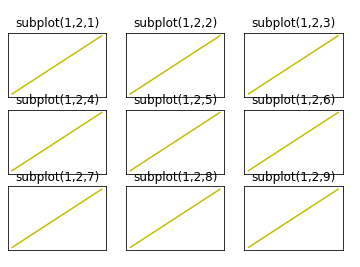
\includegraphics[width=12cm]{figures/6/1174086/subplot.png}
	\centering
	\caption{Hasil compile subplot menggunakan Matplotlib.}
\end{figure}

\subsubsection{Soal No. 6}
\hfill \break
Sebutkan semua parameter color yang bisa digunakan (contoh:  m,c,r,k,...  dkk)!

\begin{itemize}
	\item 'b' (blue)
	\item 'g' (green)
	\item 'r' (red)
	\item 'c' (cyan)
	\item 'm' (magenta)
	\item 'y' (yellow)
	\item 'k' (black)
	\item 'w' (white)
\end{itemize}

\subsubsection{Soal No. 7}
\hfill \break
Jelaskan bagaimana cara kerja dari fungsi hist, sertakan ilustrasi dan gambar sendiri!

\hfill \break
Cara kerja dari fungsi hist yaitu fungsi hist akan menerima parameter yang diberikan, kemudian fungsi hist akan dieksekusi sesuai dengan parameter yang diberikan.

\hfill \break
\textbf{Kode Program}

\lstinputlisting[caption = Kode program membuat diagram menggunakan Matplotlib., firstline=46, lastline=53]{src/6/1174086/1174086.py}

\hfill \break
\textbf{Hasil Compile}

\begin{figure}[H]
	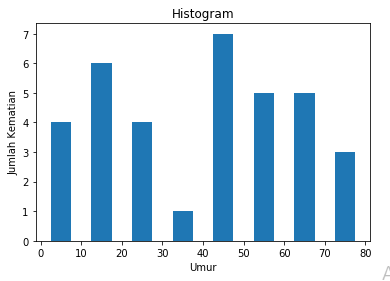
\includegraphics[width=12cm]{figures/6/1174086/histogram.png}
	\centering
	\caption{Hasil compile membuat diagram menggunakan Matplotlib.}
\end{figure}

\subsubsection{Soal No. 8}
\hfill \break
 Jelaskan lebih mendalam tentang parameter dari fungsi pie diantaranya labels, colors, startangle, shadow, explode, autopct!
 
 \begin{itemize}
 	\item labels : untuk memberikan label di tiap persentase.
 	\item colors : untuk memberikan warna di tiap persentase.
 	\item startangle : untuk memutar plot sesuai dengan derajat yang ditentukan.
 	\item shadow : untuk memberikan bayangan pada plot.
 	\item explode : untuk memisahkan antar tiap potongan pie pada plot.
 	\item autopct : untuk menentukan jumlah angka dibelakang koma.
 \end{itemize}



%%%%%%%%%%%%%%%%%%%%%%%%%%%%%%%%%%%%%%%%%%%%%%%%%%%%%%%%%%%%%%%%%%%%%%%%%%%%%%%%%%%%%%%%%%%%%%%%%%%%%%%%%%%%%%%%%%%%%%%%%%%%%%%%%%

\section{Aulyardha Anindita | 1174054}
\subsection{Pemahaman Teori}

\begin{enumerate}

\item Fungsi Library Matplotlib\\
Matplotlib adalah salah satu modul dalam python yang digunakan untuk menggambar plot 2D dengan dengan kualitas yang tinggi. Dengan matplotlib, kita dapat membuat plots, histograms, spectra, bar charts, errorchards, scatterplots, dan masih banyak lagi. Matplotlib adalah salah satu library paling banyak digunakan oleh data science untuk menyajikan datanya ke dalam visual yang lebih baik.

\item Langkah-langkah membuat sumbu x dan y di Matplotlib
\begin{itemize}
\item Buka spyder terlebih dahulu
\item Import matplotlib
\item Selanjutnya, buat x dan y. x merupakan sumbu horizontal dan y merupakan sumbu vertikal.
\item Isi sumbu x dan y sesuai dengan data yang dinginkan
\item Jangan lupa untuk memberikan perintah show untuk menampilkan grafiknya
\end{itemize}
Contoh :\\
\lstinputlisting[firstline=8, lastline=16]{src/6/1174054/Teori/1174054.py}


\item Perbedaan fungsi dan cara pakai untuk berbagai jenis plot di Matplotlib
\begin{itemize}
\item Line, Line berfungsi untuk membuat grafik sederhana yang digambar menggunakan garis biasa. Cara penggunaannya yaitu dengan menggunakan plt.plot. Untuk lebih jelasnya seperti berikut:\\
\lstinputlisting[firstline=28, lastline=33]{src/6/1174054/Teori/1174054.py}

\item Bar, Bar berfungsi untuk membuat grafik yang biasanya berbentuk kolom dan terkadang disusun baik secara vertikal maupun horizontal. Cara penggunaannya yaitu dengan menggunakan plt.bar seperti dibawah ini :
\lstinputlisting[firstline=18, lastline=26]{src/6/1174054/Teori/1174054.py}

\item Histogram, Histogram berfungsi untuk membuat grafik yang biasanya berbentuk batang. Cara penggunaannya yaitu dengan menggunakan plt.hist seperti dibawah ini :
\lstinputlisting[firstline=35, lastline=43]{src/6/1174054/Teori/1174054.py}

\item Scatt, Scatt berfungsi untuk membuat grafik yang biasanya berbentuk titik yang menggambarkan hubungan atau korelasi antara dua pasangan/variabel. Cara penggunaanya yaitu dengan menggunakan plt.scatter seperti dibawah ini :
\lstinputlisting[firstline=45, lastline=57]{src/6/1174054/Teori/1174054.py}

\item Stack Plot, berfungsi untuk membuat grafik garis yang hampir sama dengan line tetapi memiliki fill color sehingga antar line bisa berdekatan. Cara penggunaannya yaitu dengan menggunakan plt.stackplot seperti dibawah ini :
\lstinputlisting[firstline=59, lastline=75]{src/6/1174054/Teori/1174054.py}

\item Pie, berfungsi untuk membuat grafik yang biasanya berbentuk lingkaran. Cara penggunaannya yaitu dengan menggunakan plt.pie seperti dibawah ini :
\lstinputlisting[firstline=77, lastline=95]{src/6/1174054/Teori/1174054.py}

\end{itemize}

\item Cara Menggunakan Legend dan Label\\
Legend biasanya digunakan untuk mempermudah dalam membaca suatu grafik karena berisi isi dari grafik tersebut seperti nama, dan lain sebagainya. Sedangkan pada label biasanya digunakan untuk membedakan nama titik X dan titik Y. Untuk cara penggunannya seperti dibawah ini :\\
\lstinputlisting[firstline=22, lastline=24]{src/6/1174054/Teori/1174054.py}

\item Fungsi, Cara Kerja, Ilustrasi dan Parameter Pada Subplot\\
\begin{itemize}
\item Fungsi dari Subplot adalah mampu membuat grafik lebih dari satu dalam sebuah program
\item Cara Kerja dari Subplot bisa dilihat pada list berikut :\\
\lstinputlisting[firstline=97, lastline=108]{src/6/1174054/Teori/1174054.py}
\item Untuk parameternya sendiri disini saya menggunakan x dan y dimana x sebagai koordinat x dan y sebagai koordinat y.
\end{itemize}
\begin{figure}[H]	
    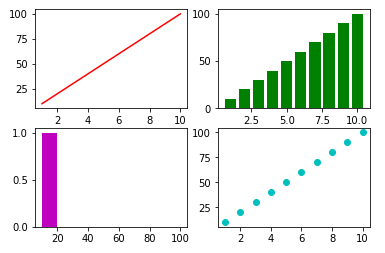
\includegraphics[width=5cm]{figures/6/1174054/Teori/subplot.png}
    \centering
    \caption{Subplot Dita}
\end{figure}

\item Parameter Color
\begin{itemize}
\item R Untuk warna merah
\item G Untuk warna hijau
\item B Untuk warna biru
\item W untuk warna putih
\item Y Untuk warna kuning
\item C Untuk warna cyan atau biru muda
\item M Untuk warna magenta
\item K Untuk warna hitam
\end{itemize}

\item Cara Kerja dan Ilustrasi Fungsi Hist\\
Cara Kerja fungsi hist ini memiliki kedua titik koordinat dimana jika nilai x misalnya adalah 9 sedangkan nilai y adalah 3 itu tidak akan terjadi masalah karena diagram ini digunakan untuk mendata data yang memiliki rentang waktu tertentu.
\begin{figure}[H]	
    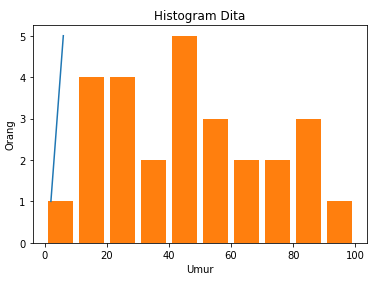
\includegraphics[width=5cm]{figures/6/1174054/Teori/histogram.png}
    \centering
    \caption{Histogram Dita}
\end{figure}

\item Parameter dari fungsi Pie
\begin{itemize}
\item Label, digunakan untuk mempermudah pembaca dalam membaca diagram pie
\item Color, digunakan untuk memberikan style atau mempermudah membaca data karena data nya yang berbeda
\item Startangle, digunakan sebagai sudut untuk memulai diagram pie
\item Shadow, digunakan untuk membuat bayangan dari diagram pie sehingga datanya terlihat menonjol
\item Explode, digunakan untuk mengeluarkan sebuah data sehingga data tersebut dapat terlihat menonjol
\item Autopct, digunakan sesuai dengan berapa angka dibelakang koma yang kita inginkan.
\end{itemize}

\end{enumerate}

%%%%%%%%%%%%%%%%%%%%%%%%%%%%%%%%%%%%%%%%%%%%%%%%%%%%%%%%%%%%%%%%%%%%%%%%%%%%%%%%%%%%%%%%%%%%%%%%%%%%%%%%%%%%%%%%%%%%%%%%%%%%%%%%%%%%

\section{Nurul Izza Hamka | 1174062 | Teori}
\begin{enumerate}

\item Fungsi Library Matplotlib\\

Matplotlib adalah Library plotting dengan 2D pada Python yang dapat Menghasilkan sebuah gambar, 
matplotlip ini paling banyak dingunakan oleh data science karena idalamnya terdapat berbagai format hardcopy dan sangat interaktif di flatformnya, 
serta mampu menyajikan visual data yang lebih baik. \\
dengan matplotlib kita dapat membuat sebuah plots,histograms, bar charts, spectra, daln lainnya.\\

\item Langkah-langkah Membuat Sumbuh X dan Y di Matplotlib

\begin{enumerate}
\item Buat plot untuk sebuah garis
\item Lakukan Import
\lstinputlisting[firstline=7, lastline=16]{src/6/1174062/Teori/1174062.py}
\end{enumerate}

\item Bagaimana Perbedaan Fungsi dan Cara Pakai Untuk Berbagai Jenis Plot Di Matplotlip

\begin{enumerate}
\item Histogram \\
Histogram menunjukkan frekuensi pada sumbu vertikal dan sumbu horizontal adalah dimensi lain. 
Histogram Ini akan menampilkan sebuah frekuensi data dengan model batang , yang mana angka didalamnya di kelompokkan dalam rentang tertentu.
\item Scatter\\
Matplotlip memiliki fungsi  untuk membuat scatterplot yang disebut scatter (). 
Plot scatter adalah jenis plot yang menunjukkan data sebagai kumpulan poin. Posisi suatu titik tergantung pada nilai dua dimensi, 
di mana setiap nilai adalah posisi pada dimensi horizontal atau vertikal.
\item Line\\
Garis dapat memiliki kedua gaya garis padat yang menghubungkan semua simpul, dan penanda di setiap titik. 
\end{enumerate}

\item Bagaimana Cara Menggunakan Legend Dan Label Serta Kaitannya Dengan Fungsinya

Formatting plot adalah suatu cara untuk memberikan sebuah informasi tentang label dan legend pada sebuah grafik dalam plot.\\
Tambahkan label = ke masing-masing plot Anda () panggilan, dan kemudian panggil legenda (loc = 'kiri atas'). 
dan kemudian memanggil kapak bukannya plt.gca (). Plot sederhana untuk kurva sinus dan cosinus dengan legend. 
Kemudian cukup tambahkan Pyplot.legend () ke bagian bawah skrip Anda dan legenda akan menampilkan label ini.

\lstinputlisting[firstline=17, lastline=21]{src/6/1174062/Teori/1174062.py}

\item Apa fungsi Dari Subplot di Matplotlip, dan Bagaimana Cara Kerja Dari Fungsi Subplot, Sertakan Ilustrasi dan Gambaar sendiri dan 
Apa Parameternya Jika Ingin Menggambar dengan 9 Subplot di Dalamnya.

Fungsi Subplot pada Matplotlib adalah kita dapat memanggil () untuk memplot sebanyak dua kali ataupun lebih dalam satu gambar.\\

\lstinputlisting[firstline=22, lastline=45]{src/6/1174062/Teori/1174062.py}
Ilustrasi 9 Gambar Subplot:
	\begin{figure}[ht!]
	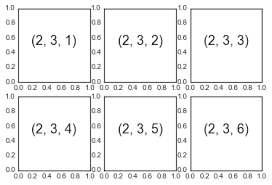
\includegraphics[width=7cm]{figures/6/1174062/subplot.png}
	\centering
	\end{figure}

\item Sebutkan parameter color yang bisa digunakan:
Matplotlib mengenali format berikut untuk menentukan warna:\\
\begin{enumerate}
\item tuple RGB yaitu {'r', 'g', 'b'}
	- {'tab:red','tab:green','tab:blue'}
\item Tuple CMYK yaitu {'c', 'm', 'y','k'}
	- {'tab:cyan','tab:magenta','tab:yellow','tab:black'}; 
\end{enumerate}

\item Bagaimana Cara Kerja Dari Fungsi Hist, sertakan Ilustrasi Dan Gambar Sendiri.\\

Pada histogram kedua titik koordinat boleh tidak sama, Misalnya X mempunyai 10 nilai sedangkan Y nya ada 5 nilai, 
karena diagram ini digunakan untuk mendata usia dari rentang tertentu atau kebutuhan lainnya.
Contoh dari penggunaan histogram :
\lstinputlisting[firstline=46, lastline=55]{src/6/1174062/Teori/1174062.py}

Ilustrasi Gambar :
	\begin{figure}[ht!]
	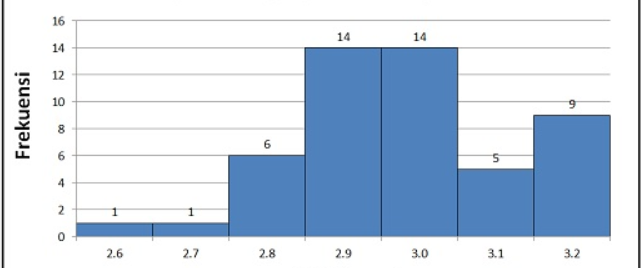
\includegraphics[width=5cm]{figures/6/1174062/histogram.png}
	\centering
	\end{figure}


\item Penjelasan tentang Parameter dari Fungsi Pie Diantaranya Labaels, Colors, Startangle, Shadow, Explode, Autopct.

\begin{enumerate}
\item Labels
Urutan string yang memberikan label untuk setiap irisan,Jumlah label harus sama dengan jumlah elemen.
\item Colors \\
Urutan warna matplotlib berargumentasi di mana diagram lingkaran akan berputar. Jika Tidak Ada, akan menggunakan warna dalam siklus aktif saat ini.
\item Startangle \\
Jika tidak ada, apakah string atau fungsi yang digunakan untuk memberi label pada irisan dengan nilai numeriknya. 
Label akan ditempatkan di dalam irisan. Jika ini adalah string format, label akan menjadi fmt persen. Jika Fungsi itu akan dipanggil.
\item Shadow \\
Gambar bayangan di bawah pai.
\item Explode \\
mengimbangi irisan dari pie.explode adalah vektor atau matriks nol dan nonzeros yang sesuai dengan Fungsi pie mengimbangi 
irisan untuk elemen bukan nol hanya dalam explode .
\item Autopct \\
autopct memungkinkan Anda untuk menampilkan nilai persen menggunakan pemformatan string Python. Dengan Autopct dan Callable kita dapat melakukan hal lebih.

\item Plagiarisme
	\begin{figure}[ht!]
	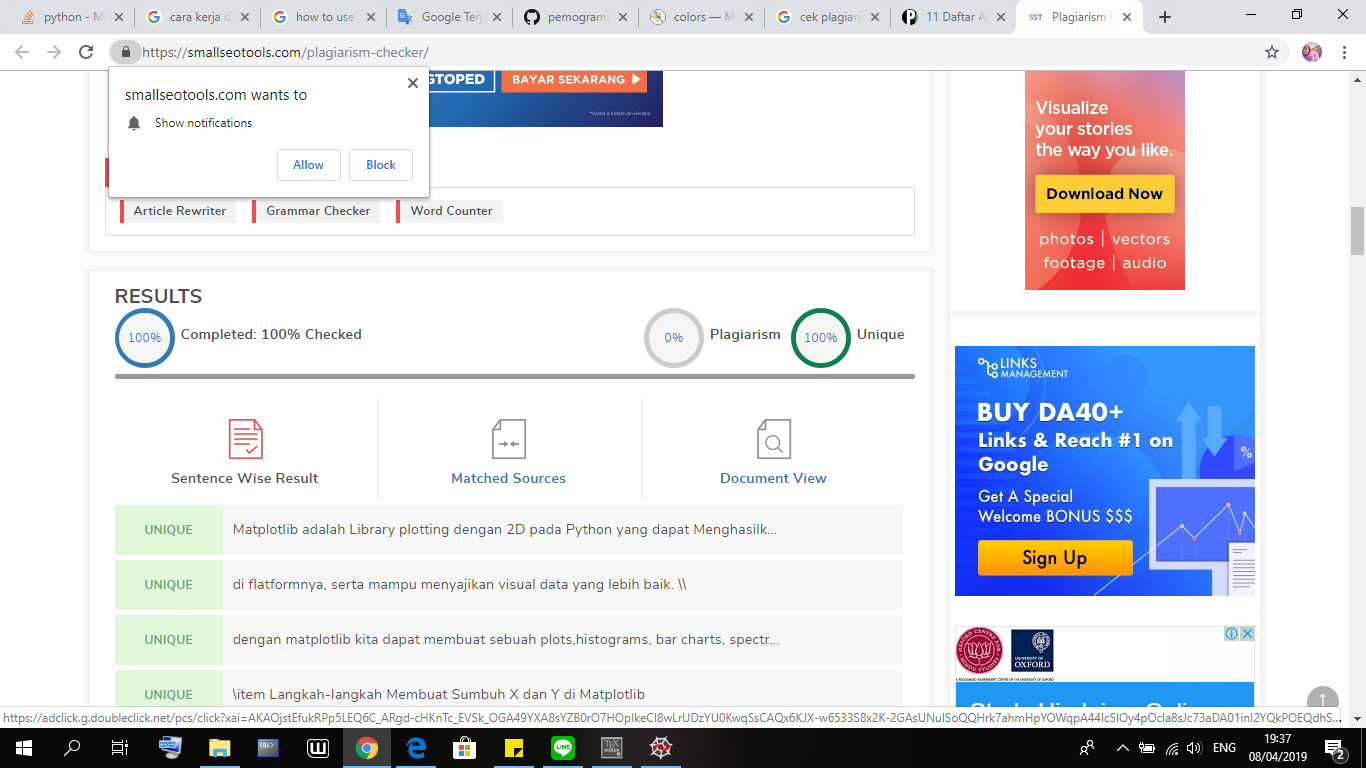
\includegraphics[width=5cm]{figures/6/1174062/plagiat.png}
	\centering
	\end{figure}

\end{enumerate}
